\chapter{Lattices and Complex Tori}
\label{ch:lattices-tori}

Let \(\omega_1,\omega_2\in\C\) be real-linearly independent.  The lattice
\[
  \Lambda=\Z\omega_1+\Z\omega_2
\]
tiles the complex plane by translates of a parallelogram.  The quotient
\[
  T=\C/\Lambda
\]
is obtained by identifying points that differ by lattice elements.

\begin{definition}
The complex torus associated to \(\Lambda\) is the quotient group
\(T=\C/\Lambda\), equipped with the complex structure induced from small disks in
\(\C\).
\end{definition}

Addition in \(\C\) descends to addition on \(T\):
\[
  [u]+[v]=[u+v].
\]
This is the analytic group law.  It is associative, commutative, and has identity
\([0]\) because those facts were true before quotienting.

\begin{proposition}
\label{prop:torus-surface}
The quotient \(T=\C/\Lambda\) is a compact genus-one Riemann surface and a
complex Lie group.
\end{proposition}

\begin{proof}
A fundamental parallelogram is compact, and its quotient maps onto \(T\), so
\(T\) is compact.  Away from identified boundary points, charts come directly
from the plane; near a boundary identification one takes a small disk whose
translates are disjoint and uses its projection.  The quotient of a parallelogram
by opposite-side identifications is a topological torus, hence genus one.
Addition is holomorphic because it is induced by the holomorphic addition map on
\(\C\).
\end{proof}

\begin{center}
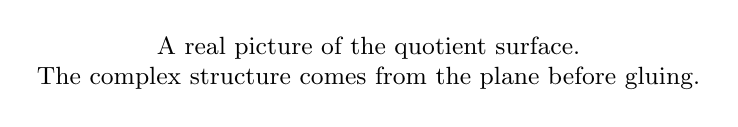
\begin{tikzpicture}[scale=0.65]
  \begin{scope}
    \drawprecisetorus
  \end{scope}
  \node[align=center, font=\small] at (0,-3.15)
    {A real picture of the quotient surface.\\The complex structure comes from
    the plane before gluing.};
\end{tikzpicture}
\end{center}

\section*{Exercises}
\addcontentsline{toc}{section}{Exercises}

\exerciseintent{Verify that addition on the quotient is independent of chosen representatives.}
\begin{exercise}
Let \(u'=u+\lambda\) and \(v'=v+\mu\) with \(\lambda,\mu\in\Lambda\).  Compute
\(u'+v'\) and show explicitly that it differs from \(u+v\) by an element of
\(\Lambda\).  Conclude that addition on \(\C/\Lambda\) is well-defined.
\end{exercise}

\exerciseintent{Check that an integral change of basis preserves the same lattice.}
\begin{exercise}
Let
\[
  \begin{pmatrix}\omega'_1\\ \omega'_2\end{pmatrix}
  =
  A\begin{pmatrix}\omega_1\\ \omega_2\end{pmatrix},
  \qquad A\in\GL_2(\Z).
\]
Use the integer entries of \(A\) and \(A^{-1}\) to prove by direct inclusion
that \(\Z\omega_1+\Z\omega_2=\Z\omega'_1+\Z\omega'_2\).
\end{exercise}

\exerciseintent{Normalize a lattice basis so its period ratio lies in the upper half-plane.}
\begin{exercise}
Let \(\tau=\omega_2/\omega_1\).  First compute why \(\operatorname{Im}\tau\ne0\).
If \(\operatorname{Im}\tau<0\), swap the basis vectors and compute
\(\operatorname{Im}(1/\tau)\).  Conclude that an oriented basis can be chosen
with \(\tau\in\HH\).
\end{exercise}

\exerciseintent{Check that torus translations are well-defined biholomorphic group translations.}
\begin{exercise}
Let \(a\in\C\).  Show that the translation map
\[
  T\longrightarrow T,\qquad [z]\longmapsto [z+a]
\]
is a well-defined biholomorphic group translation by computing what happens when
\(z\) is replaced by \(z+\lambda\), and by writing down the inverse translation.
\end{exercise}

\exerciseintent{Separate complex Lie group isomorphism from a mere abstract group isomorphism.}
\begin{exercise}
In the final theorem, the symbol \(\cong\) means isomorphism of complex Lie
groups.  Make a three-row checklist: group homomorphism, holomorphic map, and
holomorphic inverse.  For each row, write the equation or property that must be
verified beyond an abstract abelian-group isomorphism.
\end{exercise}
